\chapter{Introduction}

\paragraph*{}
This progress report aims to highlight the progress of our final project, \textbf{Collective Transport using Swarm Robotics}, with the evaluating criteria being the team individual contributions, as well as our pace in comparison to the ideal schedule. The ideal schedule can be represented by the project Gantt Chart (Figure \ref{fig:gantt_chart}).

\begin{figure}[H]
    \centering
    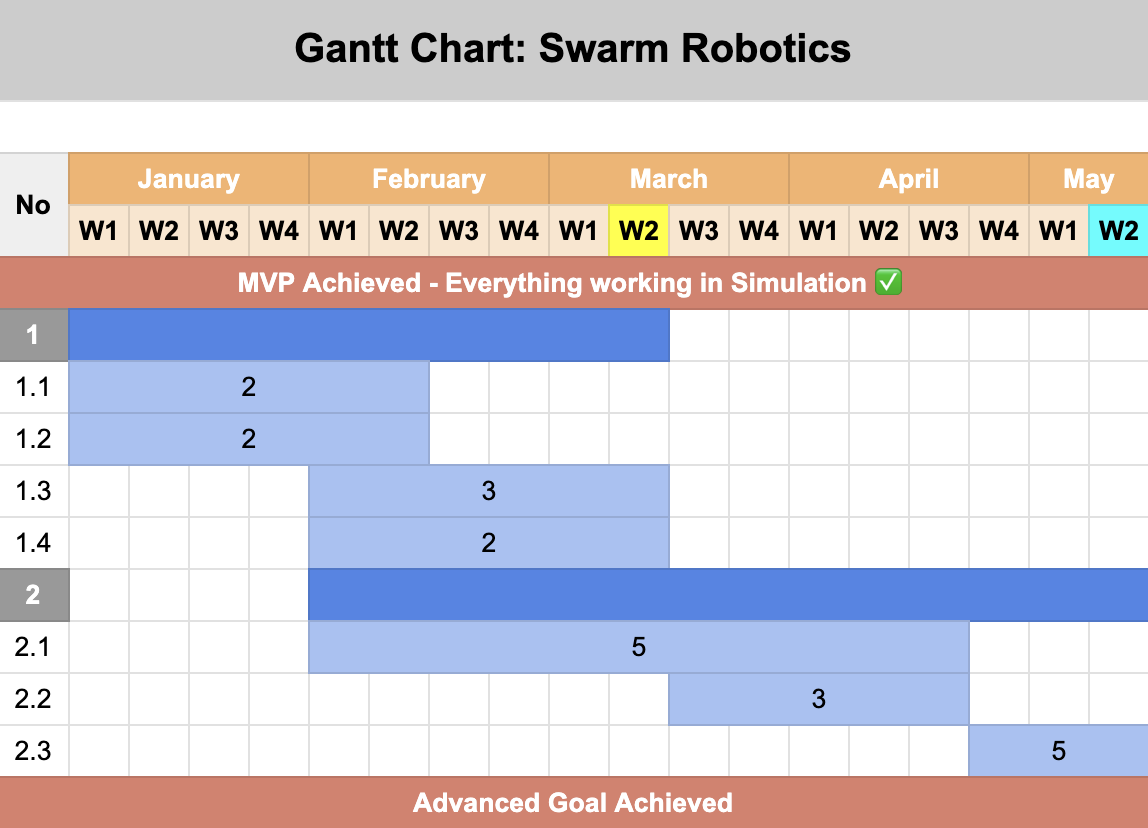
\includegraphics[width=1\linewidth]{assets/images/timeline/gantt_chart.png}
    \caption{Project Gantt Chart}
    \label{fig:gantt_chart}
\end{figure}

\paragraph*{}
According to Figure \ref{fig:gantt_chart}, we are exploring four major sub-tasks during this iteration of the project schedule. These four tasks are: \textbf{Communication in the Swarm} (Task 1.1), \textbf{Simple Simultaneous Localization and Mapping (SLAM) in Simulation} (Task 1.2), \textbf{Coordinated Gripping and Formation} (Task 1.3), and \textbf{Object detection} (Task 1.4). These tasks are planned to span from January to the second week of March. The results of the endeavors will be discussed in the following chapters


\begin{enumerate}
    \item Preparation for Hardware Implementation
    \begin{enumerate}[label=1.\arabic*]
        \item Communication in the swarm
        \item Simple Simultaneous Localization and Mapping (SLAM) in Simulation
        \item Coordinated Gripping and Formation
        \item Object detection
    \end{enumerate}
    \item Moving Towards a Complete Swarm
    \begin{enumerate}[label=2.\arabic*]
        \item Hardware
        \item Movement after Gripping
        \item Testing and Evaluation
    \end{enumerate}
\end{enumerate}

\paragraph*{}
To aid the visualization of this project. We have created a Petri Nets model (Figure \ref{fig:petri_nets}) to represent the project's workflow. Petri Nets serve as a formal modeling tool to
represent concurrent and distributed systems, providing a structured framework for analyzing complex
workflows. In the transition(rectangle) "Task Assigned from Taskmaster" force synchronization between the two dependent ask "Wait for instruction" and "Planned Path for All" to start following the planned path. For the place "Reach each destination of Yellow Cylinder \& grasp the cylinder", we can see it's connected to the transition "Task Assigned from Taskmaster" which means that the task is dependent on the taskmaster to assign the task to the robot. The transition "Task Assigned from Taskmaster" is connected to the place "Wait for instruction" which means that the robot will wait for the instruction from the taskmaster to start the task. The transition "Task Assigned from Taskmaster" is also connected to the place "Planned Path for All" which means that the robot will start following the planned path after the taskmaster assigns the task.

\begin{figure}[H]
    \centering
    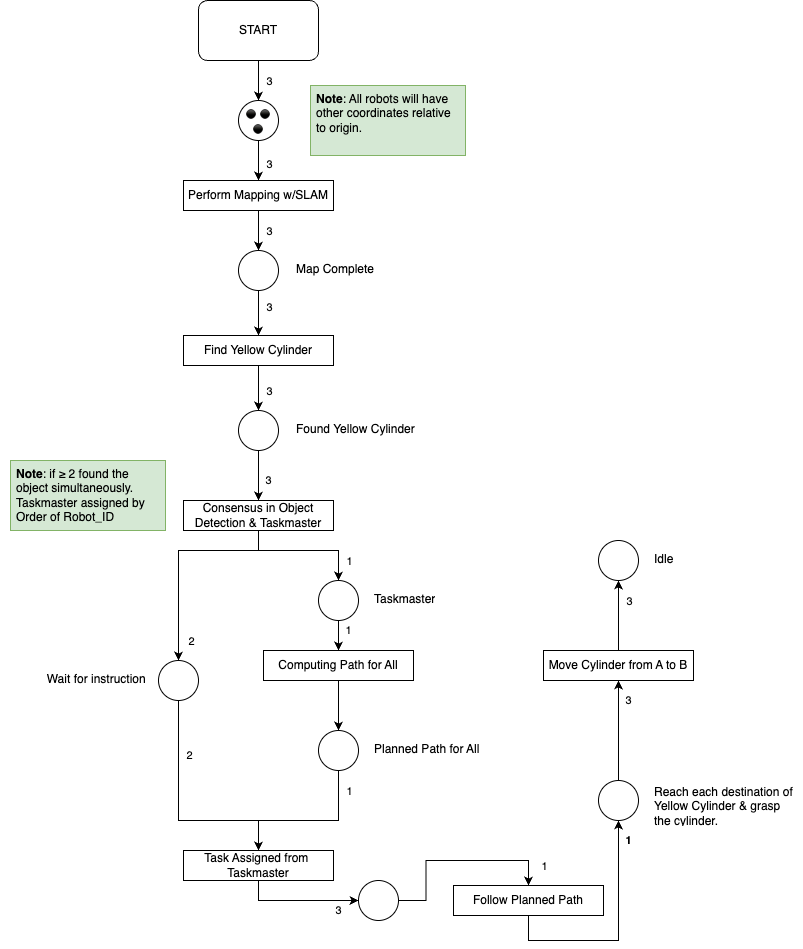
\includegraphics[width=1\linewidth]{assets/images/introduction/petri_nets.png}
    \caption{Petri Nets Model}
    \label{fig:petri_nets}
\end{figure}